\chapter{Adaptiver Gitteralgorithmus}
Mit berechenbaren Fehlerindikatoren die Verlässlichkeits- und Effizientsabschätzungen erfüllen, folgt ein Algorithmus zur effizienteren Approximation der Differentialgleichung nach dem Schema Lösen-Approximieren-Markieren-Verfeinern. Dabei entsteht eine Folge von Triangulierungen, in der von Glied zu Glied die Elemente mit den größten Indikatoren verfeinert werden.
\begin{algorithmus}[Adaptives Gitter]
	Wähle Anfangstriangulierung $\mathscr{T}_0, \theta\in (0,1],\varepsilon_{stop}>0$. Setze $k=0$.
	\begin{itemize}
		\item[(1)] Berechne Approximation $u_k\in\mathscr{S}_0^1(\mathscr{T}_k)$
		\item[(2)] Berechne Verfeinerungsindikatoren $\eta_T(u_k)$ für alle $T\in\mathscr{T}_k$
		\item[(3)] Wenn $\eta_{\mathscr{R}}(u_k) \leq \varepsilon_{stop}$, dann stopp
		\item[(4)] Wähle Menge $M_k\subset\mathscr{T}_k$ sodass
		\[ \sum_{T\in M_k} \eta_T^2(u_k) \geq \theta\sum_{T\in\mathscr{T}_k}\eta_T^2(u_k)\]
		\item[(5)] Verfeinere jedes $T\in M_k$ und anliegende Elemente, um so neue Triangulierung $\mathscr{T}_{k+1}$ zu erhalten
		\item[(6)] Setze $k \rightarrow k + 1$ und weiter mit (1)
	\end{itemize}
\end{algorithmus}
Im Schritt (5) müssen nach dem Verfeinern der Elemente in $M_k$ noch weitere Elemente verfeinert werden, um sicher zu stellen, dass eine konforme Triangulierung ohne hängende Knotenpunkte entsteht. Zudem ist es wichtig, dass die Elemente nicht degenerieren. Dafür können verschiedene Strategien verwendet werden.

\section{Rot-Grün-Blau Verfeinerung}
Der Name Rot-Grün-Blau kommt von der Bezeichnung der Aufteilungen (Abbildung \ref{dreieck}). \\ Sind alle Seiten zur Verfeinerung markiert, wird die Rot Verfeinerung angewandt. Dabei werden alle Seiten halbiert und die drei so entstandenen Knoten verbunden. Die so entstehenden Dreiecke sind vier kongruente Dreiecke und alle ähnlich zum Ausgangsdreieck mit halb so großen Seiten. \\ Sind zwei Seiten markiert, wird die Blau Verfeinerung angewandt. Dabei werden beide markierten Seiten halbiert. Die zwei so entstandenen Knoten werden verbunden genauso wie der Knoten auf der längsten Seite des Dreiecks mit dem gegenüberliegenden Knoten des Ausgangsdreiecks. \\
Ist eine Seite markiert, wird die Grün Verfeinerung angewandt. Dafür wird die längste Seite halbiert und der so entstandene Knoten mit dem Eck gegenüberliegend zur längsten Seite verbunden. \\
Da stets die längste Seite halbiert wird ist garantiert, dass die Dreiecke nicht degenerieren. Ist das Ausgangsdreieck rechtwinklig und gleichschenklig, so entstehen beim Verfeinern nur ähnliche Dreiecke.
\begin{figure}[!htbp]
	\begin{center}
		\includegraphics[width=16cm]{pics/redref.png}
	\end{center}
	\caption{\label{dreieck}Rote, grüne und blaue Verfeinerung eines Dreiecks. Die unter Kante entspricht der längsten Kante}
\end{figure}

\begin{algorithmus}[Rot-Grün-Blau Verfeinerung]
    Sei $M_k\subset \mathscr{T}_k$ Menge der zu verfeinernden Elemente.
	\begin{itemize}
		\item[(1)] Markiere alle Seiten $S \in \mathscr{S}_k$ mit $S \subset \p T, T\in M_k$
		\item[(2)] Markiere weitere Seiten, sodass für alle markierten Seiten $S\subset \p T$  auch die längste Seite von T markiert ist
		\item[(3)] Verfeinere Elemente je nach Anzahl markierter Seiten mit  Rot-,Blau- oder Grünverfeinerung für drei, zwei oder einer Seite markiert
	\end{itemize}
\end{algorithmus}

\begin{figure}[!htbp]
	\begin{center}
		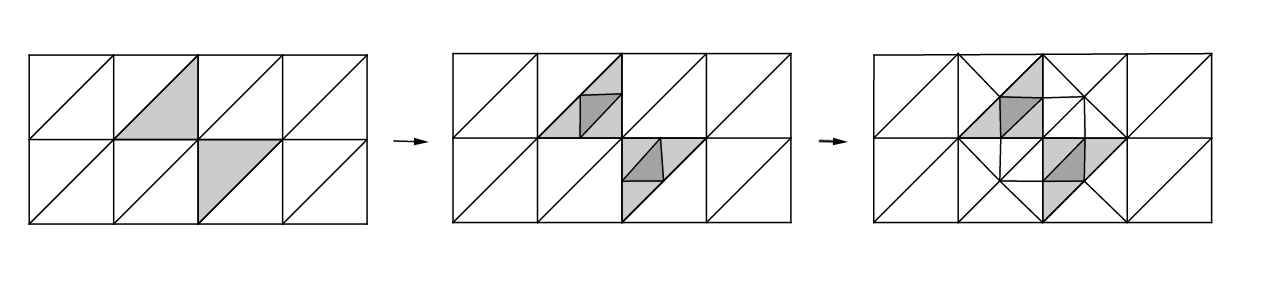
\includegraphics[width=16cm]{pics/refin.png}
	\end{center}
	\caption{Verfeinerung von markierten Elementen einer Triangulierung und weiteren Elementen, um hängende Knoten zu verhindern}
\end{figure}

\section{Bisektionsverfahren}
Eine Alternative zur Rot-Grün-Blau Verfeinerung bietet die Bisektion. Zu jedem Element wird hier eine Seite, die im nächsten Schritt halbiert werden soll, gespeichert. Im Fall der newest Vertex Bisektion in zwei Dimensionen wird jedem Element ein Verfeinerungsknoten zugeordnet. Beim Verfeinern eines Elements wird ein neuer Knoten in der Mitte der Seite gegenüber dieses Knotens erzeugt und mit dem Verfeinerungsknoten verbunden. Für die zwei so entstandenen Elemente ist der neu erzeugte Knoten der Verfeinerungsknoten (Abbildung \ref{schbisek}). Es werden dabei erst dann Elemente verfeinert, wenn die Verfeinerungsseite, also die Seite gegenüber des Verfeinerungsknotens, entweder auf dem Rand liegt oder Verfeinerungsseite des anliegenden Elements ist. So bleibt die Triangulierung in jedem Schritt regulär (Abbildung \ref{bisec}).

\begin{algorithmus}[newest Vertex Bisektion in 2d]
	Sei $d=2$ und $T\in \mathscr{T}_k$ mit Verfeinerungsseite $S$ zu verfeinerndes Element.
	\begin{itemize}
		\item[(1)] Wenn $S \subset \p \Omega$, dann erzeuge Knoten z als Mittelpunkt von S. Verbinde z mit dem Verfeinerungsknoten von T. Setze z als Verfeinerungsknoten der beiden so entstandenen Elemente. stopp  
		\item[(2)] Sei $D \in \mathscr{T}_k$ mit $D\cap T = S$. Wenn S nicht Verfeinerungsseite von D, dann wende newest Vertex Bisektion auf D an.
		\item[(3)] Erzeuge Knoten z als Mittelpunkt von S. Verbinde z mit dem Verfeinerungsknoten von T und D. Setze z als Verfeinerungsknoten der vier so entstandenen Elemente.
	\end{itemize}
\end{algorithmus}
Nach Schritt 2 ist garantiert, dass S Verfeinerungsseite von D ist. \\
Bei der newest Vertex Bisektion eines Dreiecks entstehen nur vier Ähnlichkeitsklassen, wie in Abbildung \ref{schbisek} zu sehen. Dies zeigt, dass die Dreiecke nicht degenerieren.
\begin{figure}[!htbp]
	\begin{center}
		\includegraphics[width=16cm]{pics/bisec1.png}
	\end{center}
	\caption{\label{schbisek}Schrittweise Verfeinerung eines Elements mithilfe von Bisektion und Ähnlichkeitsklassen der entstehenden Dreiecke}
\end{figure}

\begin{figure}[!htbp]
	\begin{center}
		\includegraphics[width=16cm]{pics/bisec2.png}
	\end{center}
	\caption{\label{bisec}Verfeinerung eines Elements (markiert) einer Triangulierung und weiteren Elementen, um hängende Knoten zu verhindern, mithilfe von newest Vertex Bisektion}
\end{figure}

Auch im dreidimensionalen findet das Bisektionsverfahren Anwendung. Im Gegensatz zum zweidimensionalen Analogon reicht ein Knoten jedoch nicht aus um eine eindeutige Teilung eines Elements zu bestimmen. Es kann zum Beispiel jedem Element eine Verfeinerungskante zugewiesen. Um ein Element zu teilen, wird nun ein Knoten am Mittelpunkt der Verfeinerungskante erzeugt. Die Ebene durch diesen neuen Knoten und die zwei Knoten, die der Verfeinerungskante gegenüberliegen teilt den Tetraeder in zwei neue Tetraeder. Verfahren, bei denen die neue Verfeinerungskante immer eine der beiden zum neuen Knoten gegenüberliegenden Kanten ist, werden den newest Vertex Bisektionsverfahren zugeordnet wie zum Beispiel der Algorithmus von Kossaczky (Abbildung \ref{kos}).

\begin{figure}[!htbp]
\begin{center}
	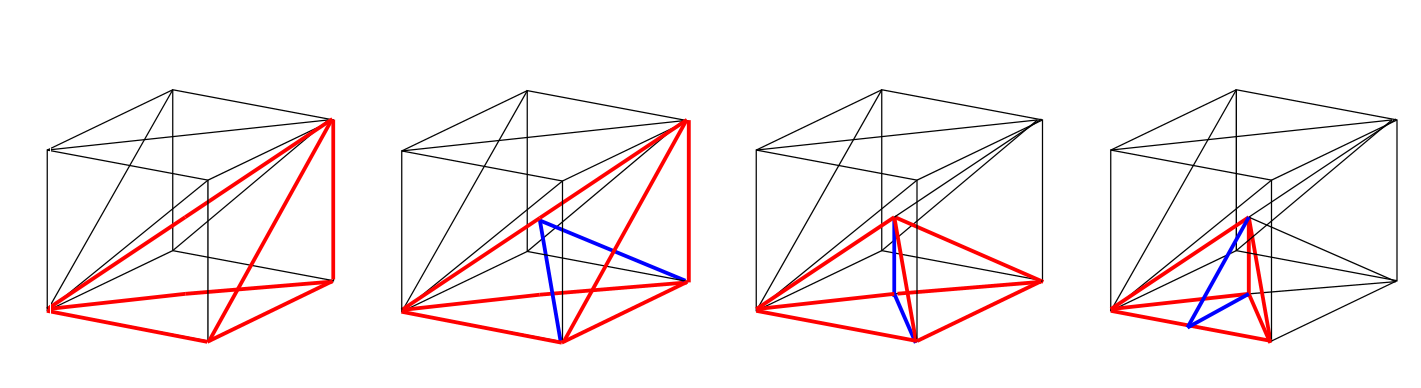
\includegraphics[width=16cm]{pics/bisec3.png}
\end{center}
\caption{\label{kos}Verfeinerung eines Tetraeders beginnend mit sechs Tetraedern mithilfe des Algorithmus von Kossaczky}
\end{figure}